\documentclass{article}

\usepackage[T1]{fontenc}
\usepackage{textcomp}

\usepackage[english]{babel}
\usepackage[utf8]{inputenc}

\usepackage{lmodern}

\usepackage{hyperref}
\hypersetup{breaklinks}
\hypersetup{pdfborder=0 0 0}

\usepackage{datetime}
\newdateformat{jpmdate}{\THEDAY~\monthname[\THEMONTH] \THEYEAR}
\AtBeginDocument{\jpmdate}

\usepackage[babel=true]{microtype}

\usepackage{amsmath}

\usepackage{geometry}

\usepackage{tikz}

\usepackage[normalem]{ulem}


\title{The impact of vector interaction with other insect species on
  disease spread}

\author{
  Elizabeth Borer
  \and
  David Crowder
  \and
  Deborah Finke
  \and
  Jing Li
  \and
  Jan Medlock
  \and
  David Pattemore
  \and
  Rakefet Sharon
}


\newcommand{\md}{\mathrm{d}}
\newcommand{\me}{\mathrm{e}}
\newcommand{\mT}{\mathrm{T}}
\newcommand{\mat}[1]{\mathbf{#1}}
\renewcommand{\vec}[1]{\mathbf{#1}}
\newcommand{\elasticity}[2]{\mathcal{E}_{#2}\negthickspace\left({#1}\right)}


\begin{document}

\maketitle

\textbf{Does the model have the gamma-distributed infection time that
  we want?}


\section{Model description}



Let $V_{ms}(t)$ and $V_{fs}(t)$ be the number of moving and feeding
susceptible vectors at time $t$, and $V_{mi}(t)$ and $V_{fi}(t)$ be
the number of moving and feeding infectious vectors at time $t$.
Likewise, let $P_s(t)$ and $P_i(t)$ be the number of susceptible and
infectious plants at time $t$.  The total number of feeding vectors is
$V_f(t) = V_{fs}(t) + V_{fi}(t)$.

Vectors are born moving.  After an exponential waiting time with mean
duration $1 / \sigma_V$, they begin feeding on a plant.  They stop
feeding and go back to the moving state after an exponential waiting
time of $1 / \tau_V$.  Feeding susceptible vectors ($V_{fs}$) can
become infected, transitioning to feeding exposed vectors ($V_{fi}$).
Once these exposed vectors start moving, they become infectious
($V_{mi}$), after which they can feed and infect plants ($V_{fi}$).

Infected vectors might lose infection at rate $\gamma_V$, which could
be set to $0$ for persistent infections.

The model is
\begin{equation}
  \label{odesystemnumbers}
  \begin{split}
    \frac{\md V_{ms}}{\md t}
    &=
    b_V V_f
    - \sigma_V V_{ms}
    + \tau_V V_{fs}
    + \gamma_V V_{mi}
    - \mu_{Vm} V_{ms}
    \\
    \frac{\md V_{fs}}{\md t}
    &=
    - \beta_V \frac{P_i}{P} V_{fs}
    + \sigma_V V_{ms}
    - \tau_V V_{fs}
    + \gamma_V V_{fi}
    - \mu_{Vf} V_{fs},
    \\
    \frac{\md V_{mi}}{\md t}
    &=
    \tau_V V_{fi}
    - \sigma_V V_{mi}
    - \gamma_V V_{mi}
    - \mu_{Vm} V_{mi},
    \\
    \frac{\md V_{fi}}{\md t}
    &=
    \beta_V \frac{P_i}{P} V_{fs}
    + \sigma_V V_{mi}
    - \tau_V V_{fi}
    - \gamma_V V_{fi}
    - \mu_{Vf} V_{fi},
    \\
    \frac{\md P_s}{\md t}
    &=
    - \beta_P V_{fi} \frac{P_s}{P} + \gamma_P P_i,
    \\
    \frac{\md P_i}{\md t}
    &=
    \beta_P V_{fi} \frac{P_s}{P} - \gamma_P P_i,
  \end{split}
\end{equation}
where $\beta_V$ is the infection rate from plants to vectors,
$\beta_P$ is the infection rate from vectors to plants, $\gamma_V$ is
the rate of pathogen clearance in vectors, $\mu_{Vf}$ is the death rate
of feeding vectors, $\mu_{Vm}$ is the death rate of moving vectors,
and $b_V$ is the birth rate of vectors.

\begin{figure}
  \centering
  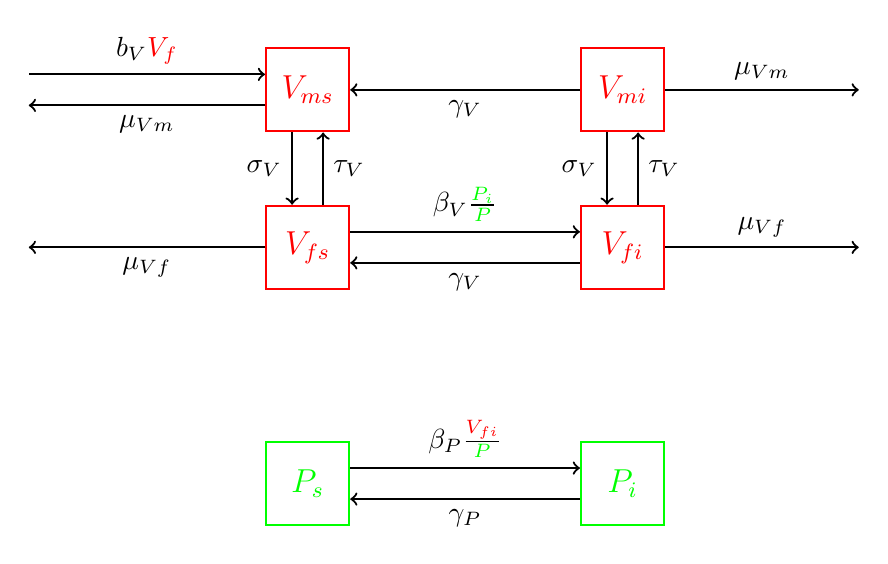
\begin{tikzpicture}[
    thick,
    scale = 1,
    %
    compartment/.style = {draw,
      font = \large,
      minimum size = {3em}},
    %
    plant/.style = {green},
    vector/.style = {red},
    ]

    \node at (0, 5)
    [compartment, vector, name = V_ms] {$V_{ms}$};
    \node at (4, 5)
    [compartment, vector, name = V_mi] {$V_{mi}$};

    \node at (0, 3)
    [compartment, vector, name = V_fs] {$V_{fs}$};
    \node at (4, 3)
    [compartment, vector, name = V_fi] {$V_{fi}$};

    \node at (0, 0)
    [compartment, plant, name = P_s] {$P_s$};
    \node at (4, 0)
    [compartment, plant, name = P_i] {$P_i$};

    \draw [->] (V_fs.20) to node [above]
    {$\beta_V \frac{\textcolor{green}{P_i}}{\textcolor{green}{P}}$}
    (V_fi.160);

    \draw [->] (P_s.20) to node [above]
    {$\beta_P \frac{\textcolor{red}{V_{fi}}}{\textcolor{green}{P}}$}
    (P_i.160);

    \draw [->] (V_mi) to node [below] {$\gamma_V$} (V_ms);
    \draw [->] (V_fi.200) to node [below] {$\gamma_V$} (V_fs.340);

    \draw [->] (P_i.200) to node [below] {$\gamma_P$} (P_s.340);

    \draw [->] (V_ms.250) to node [left] {$\sigma_V$} (V_fs.110);
    \draw [->] (V_mi.250) to node [left] {$\sigma_V$} (V_fi.110);

    \draw [->] (V_fs.70) to node [right] {$\tau_V$} (V_ms.290);
    \draw [->] (V_fi.70) to node [right] {$\tau_V$} (V_mi.290);

    \draw [<-] (V_ms.160) to node [above]
    {$b_V \textcolor{red}{V_f}$}
    +(180: 3);

    \draw [->] (V_fs.180) to node [below] {$\mu_{Vf}$} +(180: 3);
    \draw [->] (V_fi) to node [above] {$\mu_{Vf}$} +(0: 3);
    \draw [->] (V_ms.200) to node [below] {$\mu_{Vm}$} +(180: 3);
    \draw [->] (V_mi) to node [above] {$\mu_{Vm}$} +(0: 3);

  \end{tikzpicture}
  \caption{Model diagram.}
\end{figure}


Let $r$ be the level of interaction of the vector species with the
other insect species, with $r = 0$ being no interaction.  Initially,
we will consider just this implicit representation of the 2nd insect
species, but later we will explicitly model this population as well.

% The total number of vectors is
% \begin{equation}
%   V = V_{ms} + V_{fs} + V_{mi} + V_{fi},
% \end{equation}
% and its derivative is
% \begin{equation}
%   \frac{\md V}{\md t} = \left(b_V - \mu_{Vf}\right) V_f - \mu_{Vm} V_m.
% \end{equation}
% Then the fractions of vectors and plants in the various states,
% $v_{xy} = V_{xy} / V$ and $p_z = P_z / P$, are governed by the system
% of equations
% \begin{equation}
%   \label{odesystem}
%   \begin{split}
%     \frac{\md v_{ms}}{\md t}
%     &=
%     b_V v_f
%     - \sigma_V v_{ms}
%     + \tau_V v_{fs}
%     + \gamma_V v_{mi}
%     - \mu_{Vm} v_{ms}
%     - \left[\left(b_V - \mu_{Vf}\right) v_f - \mu_{Vm} v_m \right] v_{ms},
%     \\
%     \frac{\md v_{fs}}{\md t}
%     &=
%     - \beta_V p_i v_{fs}
%     + \sigma_V v_{ms}
%     - \tau_V v_{fs}
%     + \gamma_V v_{fi}
%     - \mu_{Vf} v_{fs}
%     - \left[\left(b_V - \mu_{Vf}\right) v_f - \mu_{Vm} v_m \right] v_{fs},
%     \\
%     \frac{\md v_{mi}}{\md t}
%     &=
%     \tau_V v_{fi}
%     - \sigma_V v_{mi}
%     - \gamma_V v_{mi}
%     - \mu_{Vm} v_{mi}
%     - \left[\left(b_V - \mu_{Vf}\right) v_f - \mu_{Vm} v_m \right] v_{mi},
%     \\
%     \frac{\md v_{fi}}{\md t}
%     &=
%     \beta_V p_i v_{fs}
%     + \sigma_V v_{mi}
%     - \tau_V v_{fi}
%     - \gamma_V v_{fi}
%     - \mu_{Vf} v_{fi}
%     - \left[\left(b_V - \mu_{Vf}\right) v_f - \mu_{Vm} v_m \right] v_{fi},
%     \\
%     \frac{\md V}{\md t}
%     &=
%     \left[\left(b_V - \mu_{Vf}\right) v_f - \mu_{Vm} v_m \right] V,
%     \\
%     \frac{\md p_s}{\md t}
%     &= - \beta_P v_{fi} V p_s + \gamma_P p_i,
%     \\
%     \frac{\md p_I}{\md t}
%     &= \beta_P v_{fi} V p_s - \gamma_P p_i.
%   \end{split}
% \end{equation}


\section{Pathogen growth rate}

The infected states are
\begin{equation}
  \vec{u} =
  \begin{pmatrix}
    V_{mi} \\ V_{fi} \\ P_i
  \end{pmatrix}.
\end{equation}
System \eqref{odesystemnumbers} can be written as
\begin{equation}
  \label{scriptF}
  \frac{\md \vec{u}}{\md t}
  =
  \mathcal{F}(\vec{u})
  =
  \begin{pmatrix}
    \tau_V V_{fi}
    - (\sigma_V + \gamma_V + \mu_{Vm}) V_{mi}
    \\
    \beta_V \frac{V_{fs}}{P} P_i
    + \sigma_V V_{mi}
    - (\tau_V + \gamma_V + \mu_{Vf}) V_{fi}
    \\
    \beta_P V_{fi} \frac{P_s}{P} - \gamma_P P_i
  \end{pmatrix}.
\end{equation}

The disease-free equilibrium is
\begin{equation}
  \begin{split}
    V_{ms} &=
    \\
    V_{fs} &= 
    \\
    V_{me} &= 0,
    \\
    V_{mi} &= 0,
    \\
    V_{fi} &= 0,
    \\
    P_s &= P,
    \\
    P_i &= 0.
  \end{split}
\end{equation}
Linearizing \eqref{scriptF} at the disease-free equilibrium gives
\begin{equation}
  \begin{split}
    \mat{F} &=
    \begin{bmatrix}
    - (\sigma_V + \gamma_V + \mu_{Vm}) & \tau_V & 0
    \\
    \sigma_V & - (\tau_V + \gamma_V + \mu_{Vf}) &  \beta_V
    \frac{V_{fs}}{P}
    \\
    0 & \beta_P & - \gamma_P
    \end{bmatrix}.
  \end{split}
\end{equation}
The leading eigenvalue of $\mathbf{F}$ is
\begin{equation}
  r_0 = 
\end{equation}


\section{Increasing $n$}

We are initially thinking that the effects of the second insect
species will be on vector birth rate, vector death rate, and vector
movement rate.  We will take these to have constant semi-elasticity
for simplicity for now:
\begin{equation}
  \begin{split}
    b_V(n) &= \overline{b_V} \me^{\epsilon_{b_V} n},
    \\
    \mu_V(n) &= \overline{\mu_V} \me^{\epsilon_{\mu_V} n},
    \\
    \tau_V(n) &= \overline{\tau_V} \me^{\epsilon_{\tau_V} n}.
  \end{split}
\end{equation}

Then
\begin{equation}
  \begin{split}
    \elasticity{R_0^2}{n} &=
    \frac{1}{R_0^2} \frac{\md R_0^2}{\md n}
    \\
    &=
    \frac{\left(\gamma_V + \mu_V\right)
      \left(\sigma_V + \tau_V + \gamma_V + \mu_V\right)}
    {\tau_V}
    \frac{\md}{\md n}
    \left(
      \frac{1}{\gamma_V + \mu_V}
      \frac{\tau_V}{\sigma_V + \tau_V + \gamma_V + \mu_V}
    \right)
    \\
    &=
    \frac{\left(\gamma_V + \mu_V\right)
      \left(\sigma_V + \tau_V + \gamma_V + \mu_V\right)}
    {\tau_V}
    \frac{\partial}{\partial \mu_V}
    \left(
      \frac{1}{\gamma_V + \mu_V}
      \frac{\tau_V}{\sigma_V + \tau_V + \gamma_V + \mu_V}
    \right)
    \frac{\md \mu_V}{\md n}
    \\ & \quad\quad\quad {}
    + \frac{\left(\gamma_V + \mu_V\right)
      \left(\sigma_V + \tau_V + \gamma_V + \mu_V\right)}
    {\tau_V}
    \frac{1}{\gamma_V + \mu_V}
    \frac{\partial}{\partial \tau_V}
    \left(
      \frac{\tau_V}{\sigma_V + \tau_V + \gamma_V + \mu_V}
    \right)
    \frac{\md \tau_V}{\md n}
    \\
    &=
    - \left(
      \frac{1}{\gamma_V + \mu_V}
      +
      \frac{1}{\sigma_V + \tau_V + \gamma_V + \mu_V}
    \right)
    \mu_V \epsilon_{\mu_V}
    +
    \frac{\sigma_V + \gamma_V + \mu_V}
    {\sigma_V + \tau_V + \gamma_V + \mu_V}
    \epsilon_{\tau_V}.
  \end{split}
\end{equation}


\section{Plots to make}

\begin{itemize}
\item Persistent vs.~non-persistent
\item Movement, birth, death
\item Number of interactors
\end{itemize}

\begin{itemize}
\item $R_0$ vs.~$n$
\item $R_0$ (or $\md R_0$) vs.~$\epsilon$'s (imshow, pcolor, contour,
  etc)
\item How to balance results from sensitivities (i.e.~derivatives)
  vs.~results from choosing functional forms.
\end{itemize}

\end{document}
